\section{Empirical Evaluation}
  
In this section we compare the solutions for traffic networks modeled as a QTM
before and after the introduction of a light rail.
%
We consider both fixed-time control, i.e., a non-adaptive control plan, and optimized
adaptive control obtained by solving the
MILP~(\ref{eq:objFunc},~\ref{c:turnProb}--\ref{c:pd:holdTransit}).
%
The obtained solutions are simulated using the
LP~(\ref{eq:objFunc},~\ref{c:turnProb}--\ref{c:10}) and their total
travel time and observed delay distribution are used as comparison metrics.
%
Our hypothesis is that the optimized adaptive approach is able to mitigate the
impact of introducing light rail w.r.t.\ both metrics.
%
In the remainder of this section, we present how we compute fixed-time control plans
using CTM, the traffic networks considered in the experiments, our methodology,
and the results.






\subsection{Networks}

\begin{figure}[t!]
\centering
%  trim={<left> <lower> <right> <upper>}
\subfigure[]{
\label{fig:net:arterial}
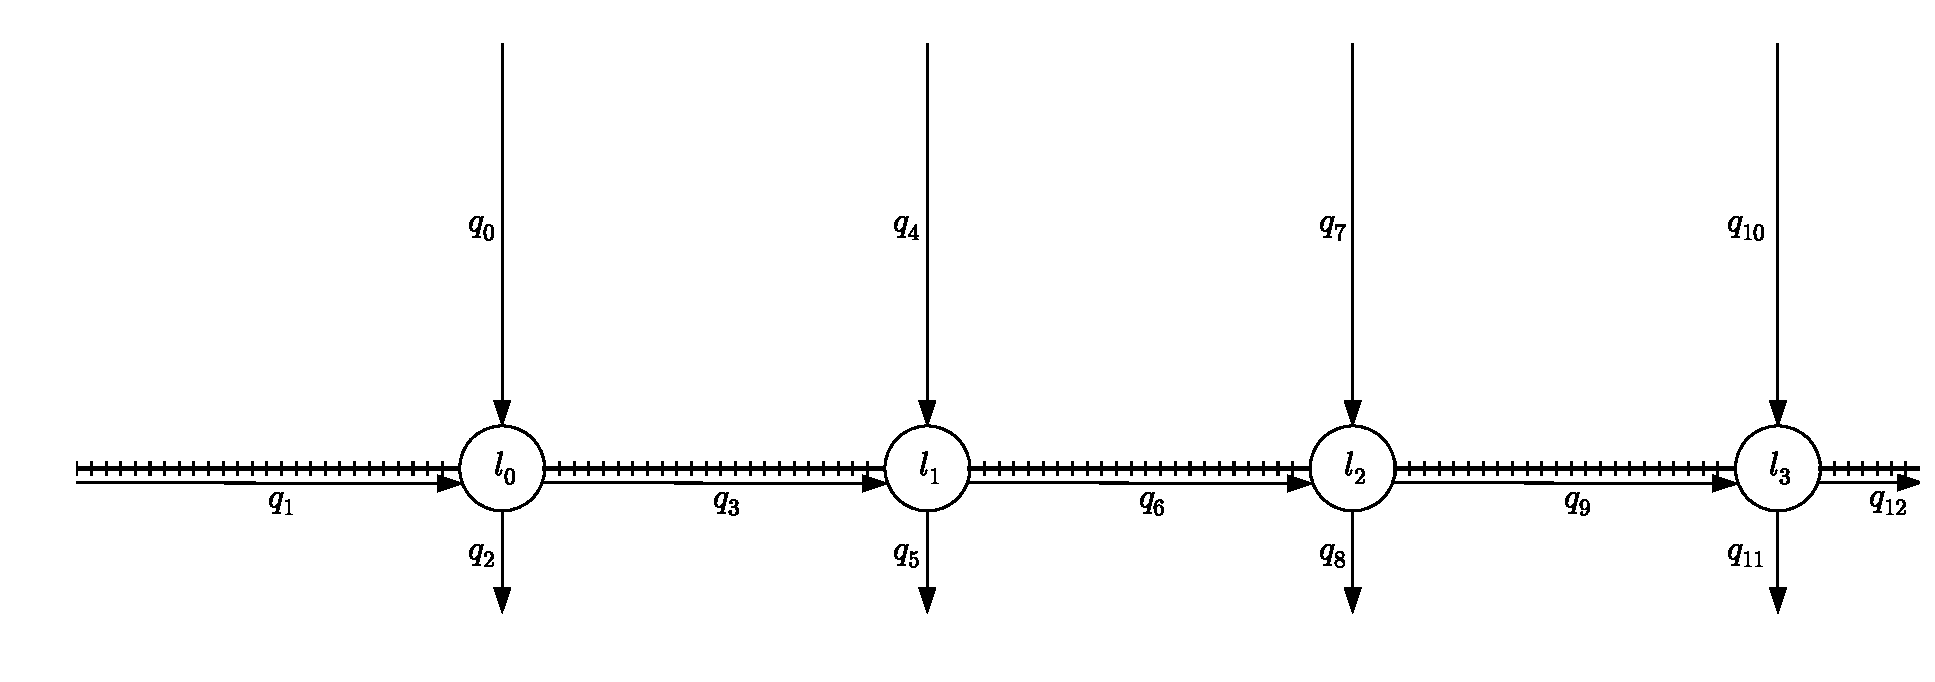
\includegraphics[trim={0 20 0 20},width=0.47\textwidth]{network1.pdf}}
\subfigure[]{
\label{fig:net:grid}
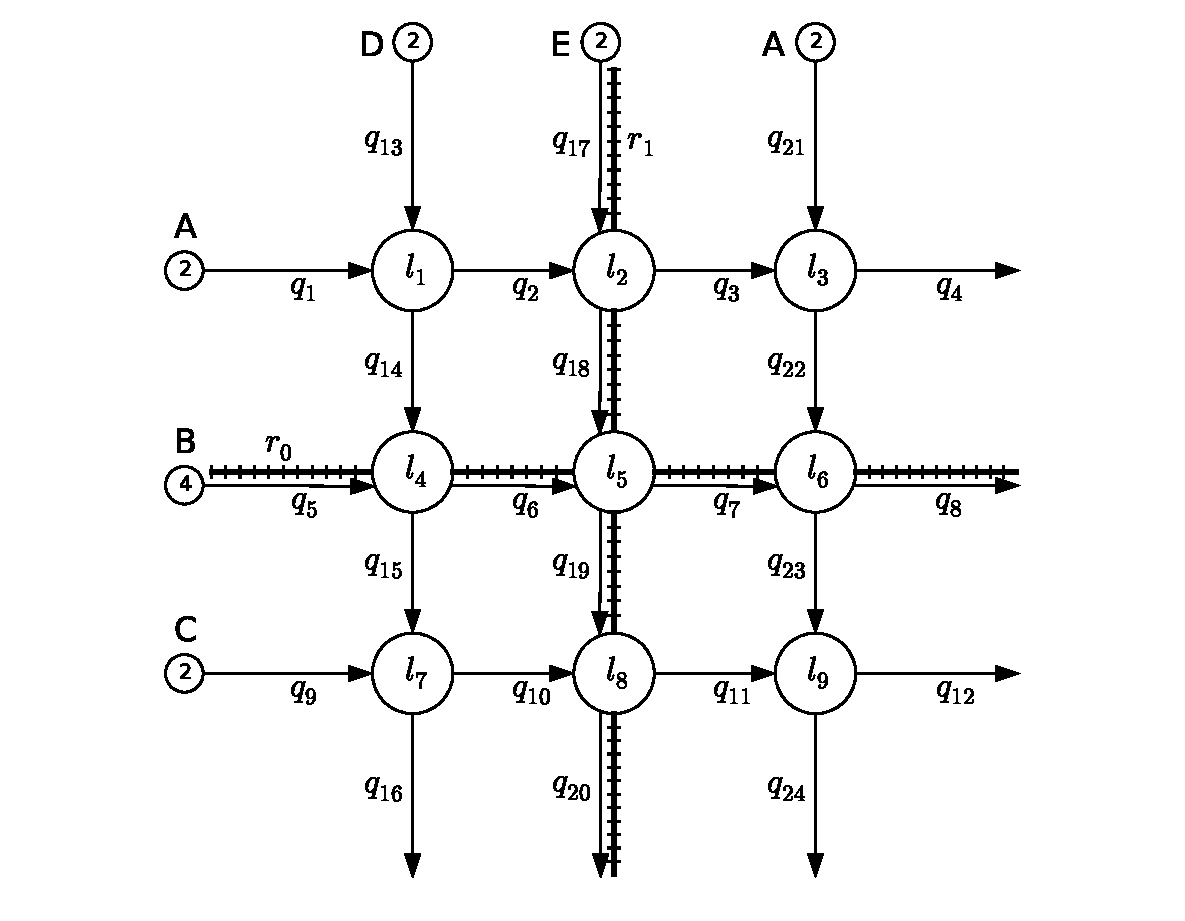
\includegraphics[trim={0 20 0 20},width=0.50\textwidth]{network2.pdf}}
\caption{Networks used to evaluate the performance:
  (a) an arterial road with parallel light rail;
  (b) an urban grid with crisscrossing streets and light rail.
%
%(d) Demand profile of the queues marked as \qLowTraf,
  %\qHighTraf, and \qVarTraf for our experiments.
}
\label{fig:networks}
\end{figure}

\begin{figure}[t!]
\centering
%  trim={<left> <lower> <right> <upper>}
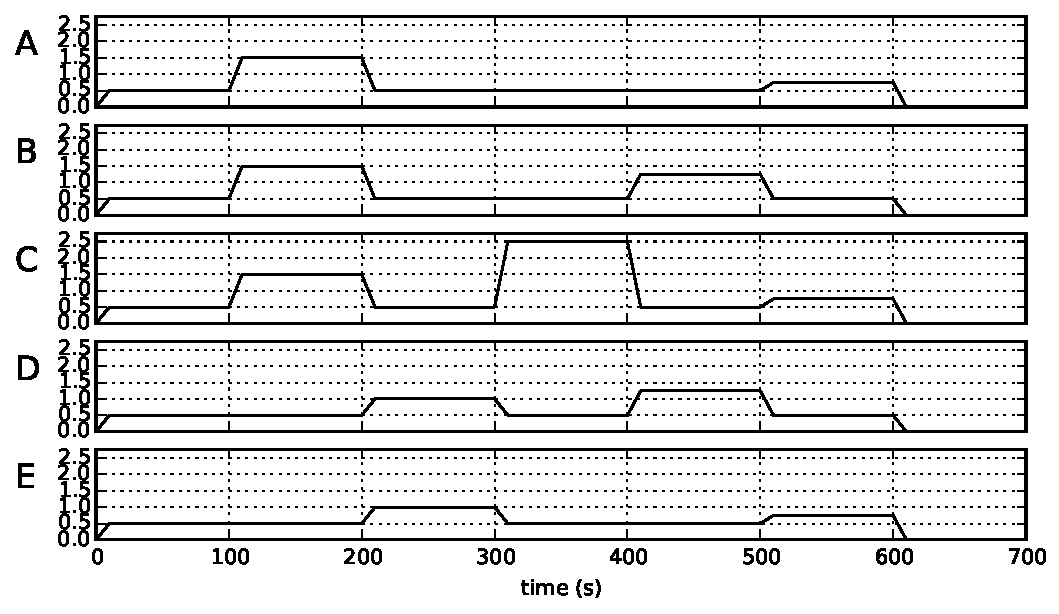
\includegraphics[width=0.47\textwidth]{demand_profiles.pdf}
\caption{Weight functions for generating demand profiles.}
\label{fig:demand_profiles}
\end{figure}

\begin{figure}[t!]
\centering
%  trim={<left> <lower> <right> <upper>}
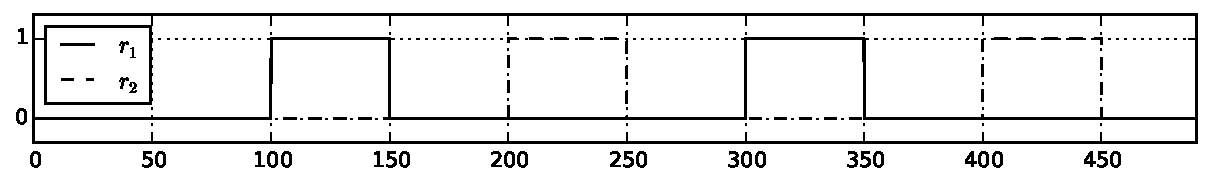
\includegraphics[trim={0 20 0 2},width=0.47\textwidth]{Transit1_sched.pdf}
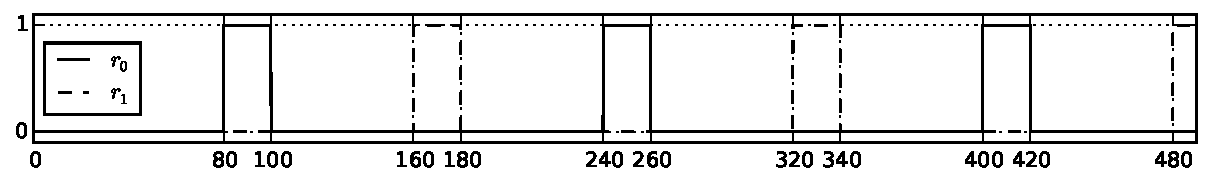
\includegraphics[width=0.47\textwidth]{Transit2_sched.pdf}
\caption{Light rail schedules.}
\label{fig:transits}
\end{figure}

We consider two networks of differing complexity: an arterial crossed by four
side streets (\cref{fig:net:arterial}) and a 3-by-3 grid (\cref{fig:net:grid}).
%
\authorHighlight{The queues receiving cars from outside of the network are
marked in \cref{fig:networks} and we refer to them as input queues.}\toIain{Make
sure to mark the new figure}
%
The maximum queue capacity~(\QMAX{i}) is 60 vehicles for non-input queues and
infinity for input queues to prevent interruption of the input demand due to
spill back from the stop line. 
%
The traversal time of each queue $i$~(\QDELAY{i}) is set at 30s,
except for the output queues on Network 1 where the traversal
time is 10s.
%
For each street, flows are defined from the head of each queue $i$ into the tail
of the next queue $j$;
%
there is no turning traffic ($\FTURN{i}{j}=1$), and the maximum flow rate
between queues, \FMAX{i}{j}, is set at 0.5 vehicles/s.
%
All traffic lights have two phases, north-south and east-west, and for all
traffic light \tl and phase $k$, \PTMIN{\tl}{k} is 10s, \PTMAX{\tl}{k} is 30s,
\CTMIN{\tl} is 20s, and \CTMAX{\tl} is 60s.


\subsection{Fixed-Time Control Constraints}

We simulate a fixed-time traffic light controller by employing the QTM to
optimize a fixed phase duration, $d^{\mathrm{fixed}}_{\ell,k}$, over the
planning horizon.
%
We implement this by replacing the bounds constraints on $\pd[n]{\ell}{k}$
($\pd[n]{\ell}{k} \le \PTMAX{\ell}{k}$ and \ref{c:minPhase}), with fixed duration
constraints, employing the \textit{big-M} method to apply the constraints only
while the phase is inactive, where 
$d^{\mathrm{fixed}}_{\ell,k} \in [\PTMIN{\ell}{k}, \PTMAX{\ell}{k}]$.
%
\begin{cAlign}
\pd{\ell}{k} &\le d^{\mathrm{fixed}}_{\ell,k} + \PTMAX{\ell}{k} \p[n]{\ell}{k}
  \tagconstrain{c:pd:fixedUB}\\
%
\pd{\ell}{k} &\ge d^{\mathrm{fixed}}_{\ell,k} - \PTMAX{\ell}{k} \p[n]{\ell}{k}
  \tagconstrain{c:pd:fixedLB}
\end{cAlign}
 
Constraints \ref{c:pd:fixedLB} and \ref{c:pd:fixedUB} are only applied for time
intervals $n$ where $\tn[n] > \CTMAX{\tl}$, to allow the controller to select an
optimized phase offset at the start of each plan.
%TODO talk about how the fixed phase times fit around transit crossings.


\subsection{Experimental Methodology}

Each network is evaluated at increasing demand levels up to the point where $\inq{i}$
becomes saturated.
%
\fnremark{FWT: we need to clarify that both approaches have access to the whole
``future'', i.e., perfect information about the incoming cars.}
%
For each demand level, traffic is injected into the network in bursts over 600s.
By setting each 
$\QIN{i}{n} = \mathrm{max}(\alpha \beta \mathrm{w}_i(\tn[n]),\beta)$, where $\mathrm{w}_i$
is a weight function in \cref{fig:demand_profiles} corresponding to the letter label in 
\cref{fig:networks}, $\beta$ is the maximum inflow rate in vehicles per \DT, as annotated at the queue input in \cref{fig:networks}, and $\alpha \in [0,2]$, is the
the scaling factor for the demand level being evaluated.
\TMAX is set sufficiently high to allow all traffic to clear the network,
typically in the range 1000s to 1500s.\toIain{check horizons}
%
By clearing the network, we can easily measure the total travel time for all the
traffic as the area between the cumulative arrival and departure curves measured
at the boundaries of the network.
%
%TODO \fnremark{FWT: is this explanation of how to compute the total travel time
%still necessary?}
%
%\cref{tab:network_demand} presents the demand profile of each network.
%

We evaluate each network using fixed time control and the optimized control in
two scenarios: before the introduction of the transit and
after. In both cases, we use \DT[] equal to 10s for all $n$. Additionally we evaluate each network 
with two different light rail schedules as shown in  \cref{fig:transits}. A slow light rail with a crossing duration of 50s
and a period of 200s, and a fast light rail with a crossing duration of 20s and period of 160s. On Network 2, the North-South schedule is
offset by 100s for the slow light rail and 80s for the fast light rail to avoid a collision at $l_5$.

For all experiments, we used Gurobi as the MILP solver running on a
heterogeneous cluster \authorHighlight{with 2.8GHz AMD Opteron~4184, 3.1GHz AMD
Opteron~4334 (12 cores each), and 2Ghz Intel Xeon E5405 (4 cores). We use 4
cores for each run of the solver.}\footnote{\authorHighlight{FWT: we can easily
cut this description in case we're 1 or 2 lines short.}}

We limit the MIP gap accuracy to 0.02\% and 0.1\% for the arterial and grid
networks, respectively.
%
Due to Gurobi's stochastic strategies, runtimes for the solver can vary,
and we do not set a time limit.
%
The optimized adaptive solution are typically found in real time, while
fixed-time plans can take significantly longer; however, once the fixed-time
solution is found, it can be deployed indefinitely.\toIain{Do you have the
cputimes by any chance in your log files so that we could say what is the
average?}




\subsection{Results}

\begin{figure*}[t!] \centering
%  trim={<left> <lower> <right> <upper>}
\subfigure[]{\label{fig:arterial:delayCurve}
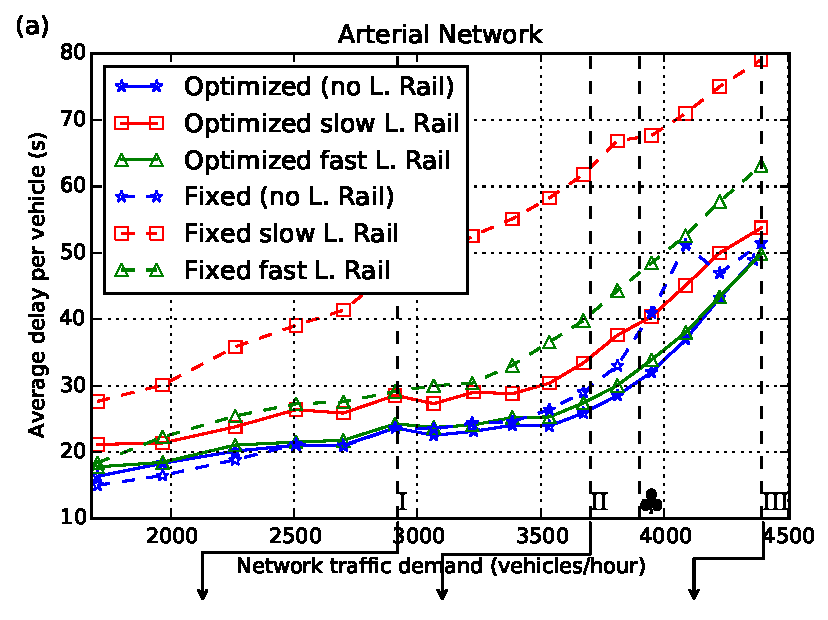
\includegraphics[keepaspectratio,width=0.49\textwidth]{network1_delay.pdf}}
\subfigure[]{\label{fig:grid:delayCurve}
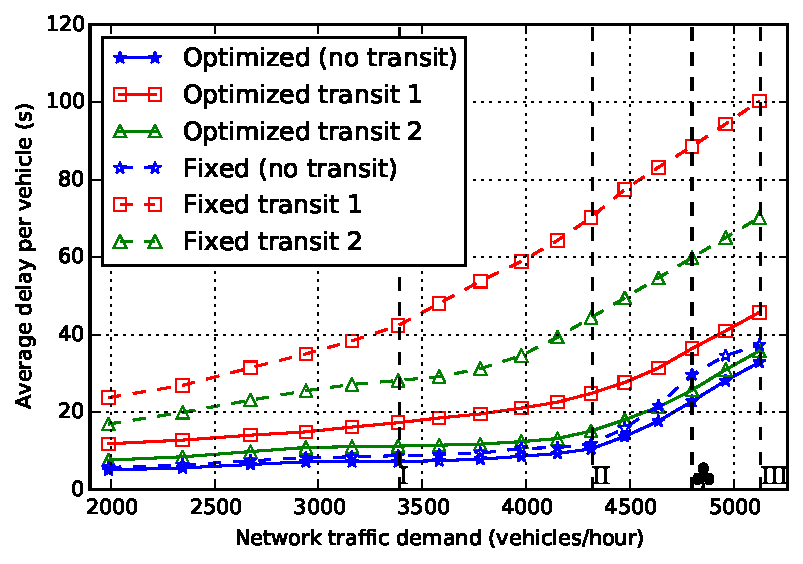
\includegraphics[keepaspectratio,width=0.49\textwidth]{network2_delay.pdf}}
\subfigure[]{\label{fig:arterial:boxplot}
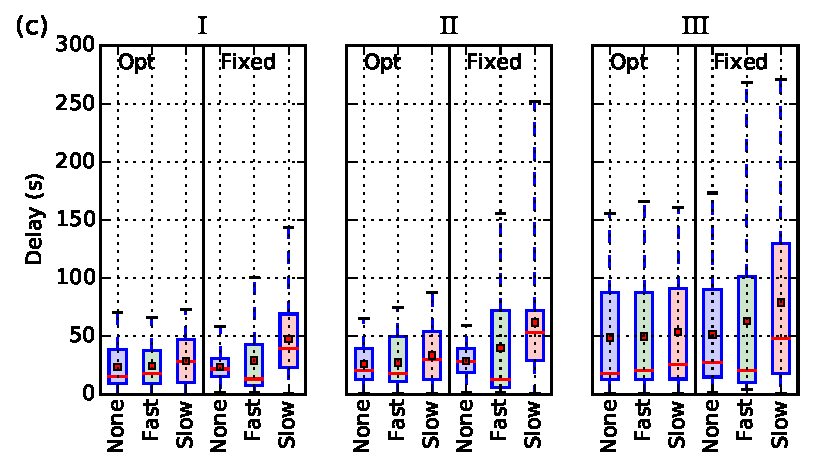
\includegraphics[keepaspectratio,width=0.49\textwidth]{network1_boxplots.pdf}}
\subfigure[]{\label{fig:grid:boxplot}
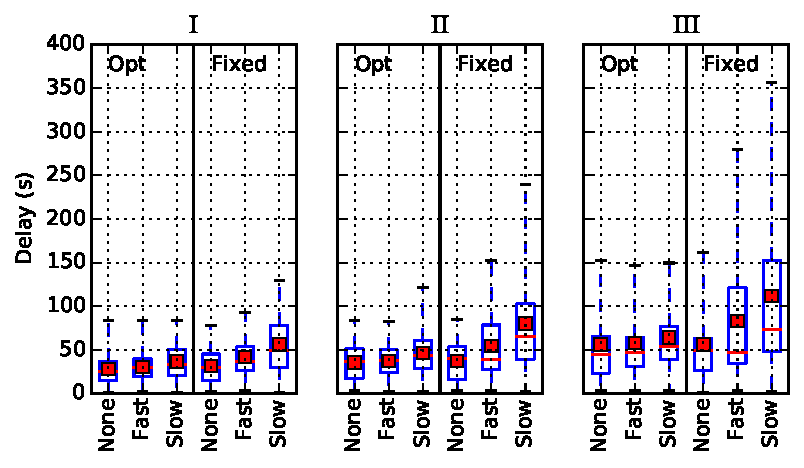
\includegraphics[keepaspectratio,width=0.49\textwidth]{network2_boxplots.pdf}}
%
\caption{Average delay by the network demand for the arterial (a) and grid (b)
networks. Box plots representing the observed distribution of delay for 3
different values of demand for each network (c,d). The mean is presented as a
red square in the box plots.}
%
\label{fig:delayCurveAndBoxplot} \end{figure*}


%


%We compare the performance of non-homogeneous and homogeneous solutions in two
%ways: comparing the decrease in total travel time with increasing major frame
%time (greater look ahead), and analysing the distribution of delay in each
%queue of the network.
%
\cref{fig:arterial:delayCurve,fig:grid:delayCurve} show, for each network, the
average delay per vehicle as a function of demand for both fixed-time and adaptive
control approached in three scenarios: before the light rail and after the
installation of a light rail using schedules 1 and 2.
%
As we hypothesized, optimized adaptive control is able to mitigate the impact of
the introduction of light rail and it marginally increases the average delay
when compared with the average delay produced by fixed-time controller
\textbf{before} the light rail.
%
Moreover, as shown in \cref{fig:arterial:boxplot,fig:grid:boxplot}, the optimized
adaptive controller also produces better quality policies than the fixed-time
controller, i.e., policies with smaller median, third quartile, and maximum
delay.
%
In our experiments, the maximum observed delay after the light rail for the
optimized adaptive policies is no more than the double of the maximum delay before
the its introduction (for both fixed and adaptive approaches).\toIain{Can you
double check this in the data?}



\begin{figure*}[t!] \centering
%  trim={<left> <lower> <right> <upper>}
\subfigure[]{\label{fig:arterial:impact:t1}
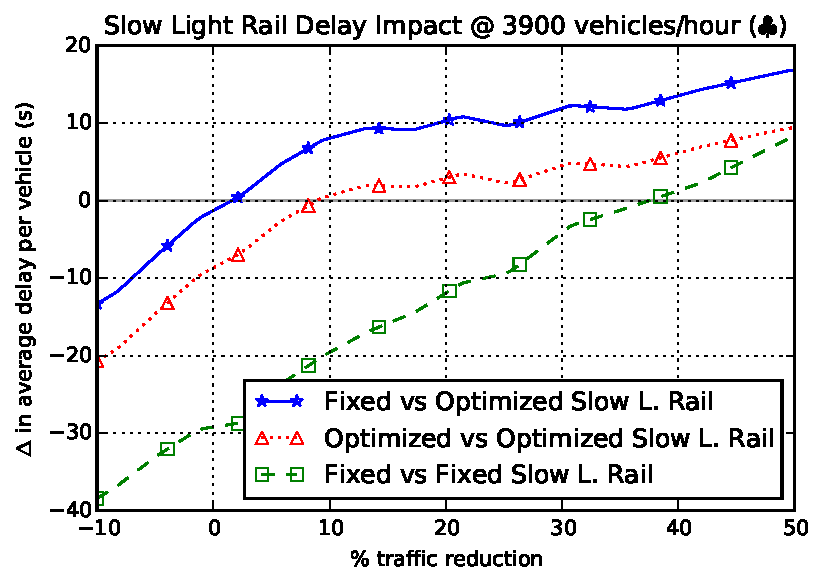
\includegraphics[keepaspectratio,width=0.49\textwidth]{network1_t1_reduction.pdf}}
\subfigure[]{\label{fig:grid:impact:t1}
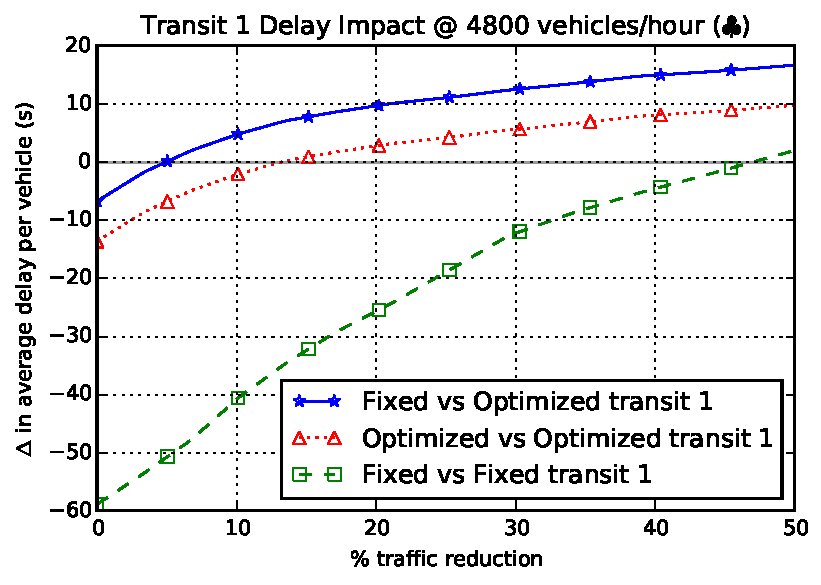
\includegraphics[keepaspectratio,width=0.49\textwidth]{network2_t1_reduction.pdf}}
\subfigure[]{\label{fig:arterial:impact:t2}
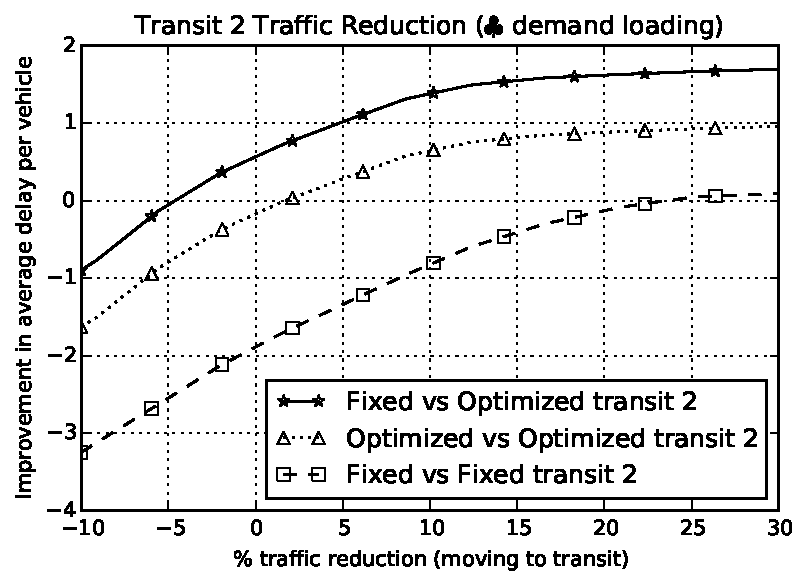
\includegraphics[keepaspectratio,width=0.49\textwidth]{network1_t2_reduction.pdf}}
\subfigure[]{\label{fig:grid:impact:t2}
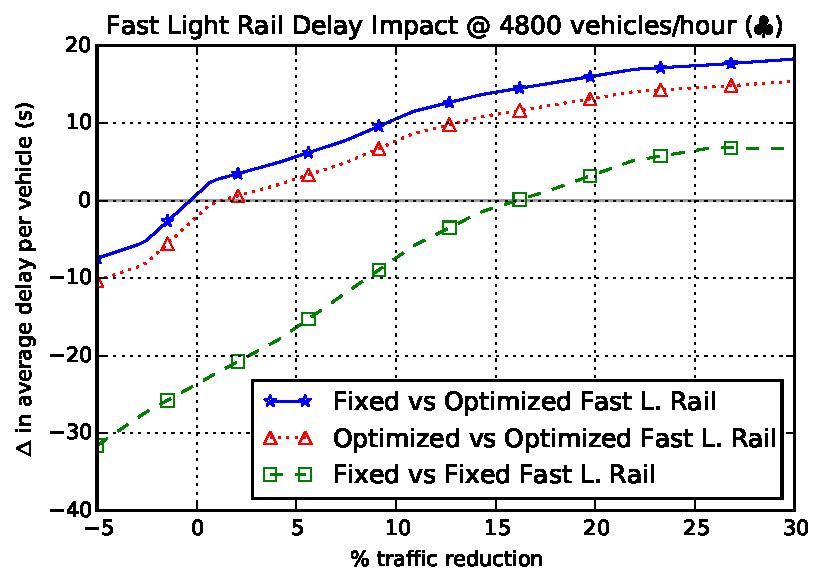
\includegraphics[keepaspectratio,width=0.49\textwidth]{network2_t2_reduction.pdf}}
%
\caption{Impact on average delay for the arterial (first column) and grid
(second column) networks for both light rail schedules (rows) in different
scenarios (curves) of traffic control system before and after installation of
light rail.
%
The x-axis is the percentage of cars that switching to the public transportation
and the y-axis is the impact after the light rail is installed.
%
Negative impact represents increase in average delay.}
%
\label{fig:impact} \end{figure*}



To further illustrate the benefits of using optimized adaptive control to minimize
the impact adding light rail to traffic network, \cref{fig:impact} shows the
impact on average delay as a function of the percentage of cars that switching
to the light rail.\fnremark{FWT: say that we are look at a fixed demand and that
this value is depicted by $\clubsuit$ in \cref{fig:delayCurveAndBoxplot}}.
%
In these plots, higher numbers are better (i.e., there is a decrease in the
average delay) and zero means that there is no change after installing light
rail.
%
For the three combinations of before and after policies presented,
%
%(we omit the case of using optimized adaptive before the light rail and
%fixed-time after the light rail),
%
we can see that, while keeping the fixed-time controller requires from 25\% to
45\% of the drives to switch to light rail in order to obtain the same average
delay as before its installation, the optimized adaptive approach requires only from
2.5\% to 10\% of the drivers to switch when already using optimized adaptive
control \textbf{before} the light rail.
%
When compared fixed-time before the light rail and optimized adaptive after, the
average delay stays the same if only the 2\% and 5\% of the drives switch to the
light rail when considering first schedule in the arterial and grid networks,
respectively;
%
moreover, the average delay \textbf{decreases} for both networks using the
second light rail schedule even if no driver switches to the newly installed
public transportation.

